\documentclass{beamer}
\usetheme{Montpellier}
\usecolortheme{dolphin}

%\usepackage{graphicx} %For jpg figure inclusion
%\usepackage{times} %For typeface
%\usepackage{epsfig}
\usepackage{color} %For Comments
\usepackage{beamerthemeshadow} %Paul and Lemmon put this in, take out if you want
%\usepackage[all]{xy}
%\usepackage{float}
%\usepackage{subfigure} 
%\usepackage{hyperref}
%\usepackage{url}
%\usepackage{parskip}
%\usepackage{multirow}

%% Elena's favorite green (thanks, Fernando!)
\definecolor{ForestGreen}{RGB}{34,139,34}
\definecolor{BlueViolet}{RGB}{138,43,226}
\definecolor{Coquelicot}{RGB}{255, 56, 0}
\definecolor{Teal}{RGB}{2,132,130}
% Uncomment this if you want to show work-in-progress comments
\newcommand{\comment}[1]{{\bf \tt  {#1}}}
% Uncomment this if you don't want to show comments
%\newcommand{\comment}[1]{}
\newcommand{\emcomment}[1]{\textcolor{ForestGreen}{\comment{Elena: {#1}}}}
\newcommand{\todo}[1]{\textcolor{blue}{\comment{To Do: {#1}}}}
\newcommand{\pscomment}[1]{\textcolor{Coquelicot}{\comment{Paul: {#1}}}}
\newcommand{\mmcomment}[1]{\textcolor{magenta}{\comment{Max: {#1}}}}
\newcommand{\escomment}[1]{\textcolor{BlueViolet}{\comment{Emma: {#1}}}}
\newcommand{\alcomment}[1]{\textcolor{red}{\comment{Lemmon: {#1}}}}
\newcommand{\hfcomment}[1]{\textcolor{Teal}{\comment{Henry: {#1}}}}
%%%%%%%%%%%%%%%%%%%%%%%%%%%%%%%%%%%%%%%%%%

\begin{document}
\title{Developing Beginner-Friendly User Interactions for the Clojure Programming Language}
\date{April 11, 2015}

\begin{frame}
\frametitle{Developing Beginner-Friendly User Interactions for the Clojure Programming Language}
{\centering
\noindent
Henry Fellows, Aaron Lemmon, Max Magnuson, \par
Emma Sax, Paul Schliep, and Elena Machkasova \par

{\it 
Midwest Instruction and Computing Symposium\par
April 11, 2015\par}
}
\end{frame}
%frame

\begin{frame}
\frametitle{Table of contents}
\tableofcontents  
\end{frame}

\section{Overview of Clojure}

\begin{frame}
\frametitle{Intro to Clojure}
	\begin{itemize}
  	 \item Fill in things here......
  	 \item \hfcomment{This probably needs to be a few slides.}
	 \end{itemize}
\end{frame}

\section{Error Messages}

\begin{frame}
\frametitle{Clojure error messages: background}
	\begin{itemize}
  		\item Error messages need to be:
  		\begin{itemize}
  	 		\item helpful for debugging
  	 		\item easy to understand
  	 		\item approachable
  		\end{itemize}
	 \end{itemize}
\end{frame}

\begin{frame}[fragile]
\frametitle{Clojure error messages: example}
	\begin{itemize}
  	 \item Fill in things here......
	 \end{itemize}
\end{frame}

\begin{frame}
\frametitle{Error message transformations: try/catch}
	\begin{itemize}
  	 \item Fill in things here......
	 \end{itemize}
\end{frame}

\begin{frame}
\frametitle{Error message transformations: function substitution}
	\begin{itemize}
  	 \item Fill in things here......
	 \end{itemize}
\end{frame}

\begin{frame}[fragile]
\frametitle{User scenarios: example}
	\begin{itemize}
  	 \item Fill in things here......
	 \end{itemize}
\end{frame}

\begin{frame}
\frametitle{User scenarios: explanation}
	\begin{itemize}
  	 \item Fill in things here......
	 \end{itemize}
\end{frame}

\begin{frame}
\frametitle{Hints: How they are helpful}
	\begin{itemize}
  	 \item Fill in things here......
	 \end{itemize}
\end{frame}

\begin{frame}
\frametitle{Hints: example}
	\begin{itemize}
  	 \item Fill in things here......
	 \end{itemize}
\end{frame}

\begin{frame}
\frametitle{Hints: future work}
	\begin{itemize}
  	 \item Fill in things here......
	 \end{itemize}
\end{frame}
% Henry & Max
\section{Technical Setup}
\begin{frame}
\frametitle{Setup}
	\begin{itemize}
		\item IDE
		\begin{itemize}
			\item LightTable
			\item Nightcode
		\end{itemize}
		\item Leiningen
		\begin{itemize}
			\item project manager
			\item popular in Clojure community
		\end{itemize}
	\end{itemize}
\end{frame}

\begin{frame}[fragile]
\frametitle{Current Workflow Diagram}
\begin{figure}[h]
 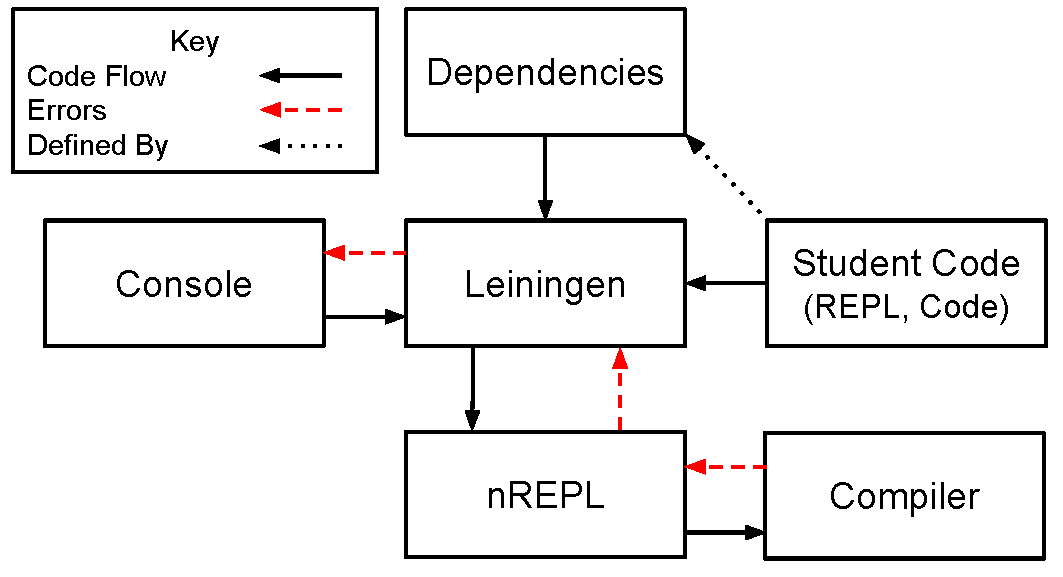
\includegraphics[width=10cm]{../CurrentErrorHandling.pdf}
 \centering
\end{figure}
\end{frame}

\begin{frame}
\frametitle{Issues 1}
	\begin{itemize}
		\item installation of Leiningen is nontrivial
		\item command line acts as a barrier
		\item we do not want students managing dependencies
		\item no integration with new error handling system
	\end{itemize} 
\end{frame}

\begin{frame}
\frametitle{Proposed Solutions}
	\begin{itemize}
		\item use scripting to abstract over Leiningen installation
		\item Graphical User Interface will abstract over command line
		\item Leiningen plugin to inject needed dependencies
		\item use nREPL to integrate new error handling system
	\end{itemize}
\end{frame}

\begin{frame}[fragile]
\frametitle{Proposed Workflow Diagram}
\begin{figure}[h]
 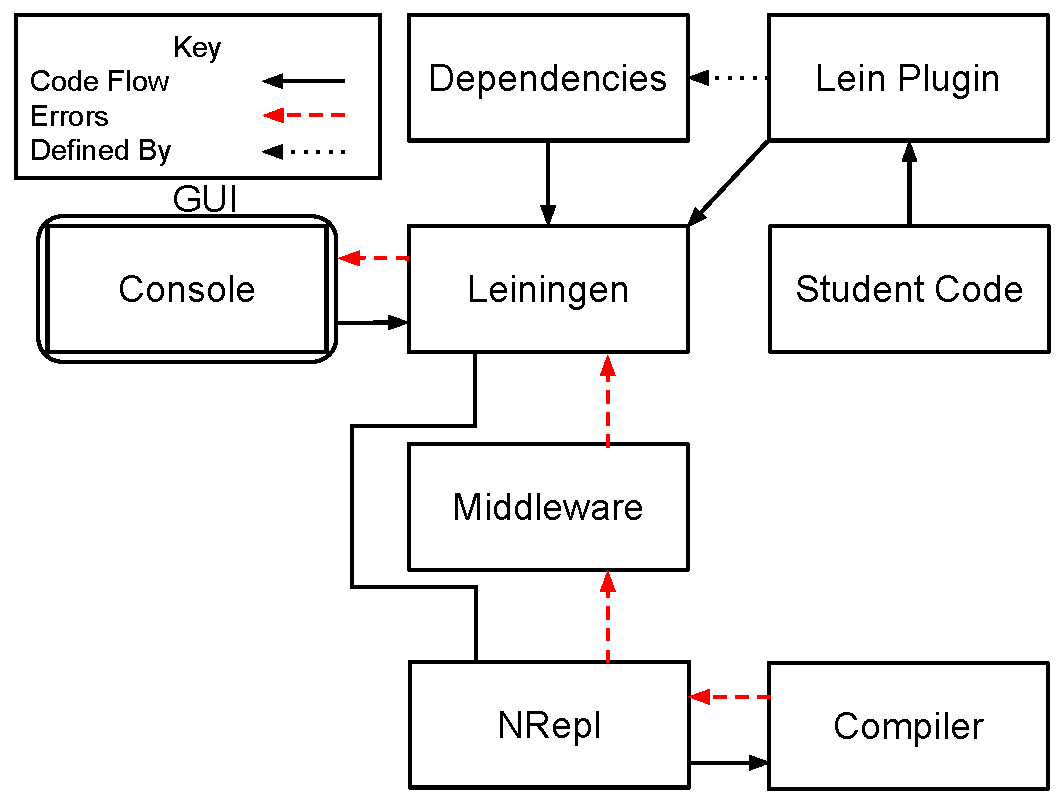
\includegraphics[width=9cm]{../OurErrorHandlingSystem.pdf}
 \centering
\end{figure}
\end{frame}

\begin{frame}
\frametitle{What needs to be done}
\end{frame}

\end{document}

